%\documentclass{beamer}
%\usetheme{Pittsburgh} 
\documentclass{scrartcl}

\usepackage[utf8]{inputenc}
\usepackage{default}
\usepackage[procnames]{listings}
\usepackage{graphicx}
%\usepackage[toc,page]{appendix}
\usepackage{caption}
\usepackage{hyperref}
\usepackage{color}

\usepackage{enumitem} 

\usepackage{pdfpages}


%Bibliogrpahy?
\usepackage{bibentry}
%\nobibliography*
%\bibentry{ }


\begin{document}

\title{Assignment No. 7}
\subtitle{}
\author{
  Quignon, Christophe \\
  %Familyname, Name
} 
\date{\today}


\maketitle

\section{Read chapter 6 from Haykin’s book}
\begin{enumerate}
\item Introduction
	\begin{itemize}
	\item SVM is a linear machine.
	\item The idea behind SVM is to construct a hyperplane to separate data.
	\item SVM is an approximate implementation of structural risk minimization
	\item SVM do not include domain knowledge
	\item The support vector is drawn by an inner kernel from the data
	\item Three types of SVM can be constructed by different kernels:
		\begin{itemize}
		\item Polynomial learning
		\item Radial-basis function networks
		\item Two-layer perceptrons
		\end{itemize}
	\end{itemize}

\item Optimal hyperplane for linearly separable patterns
	\begin{itemize}
	\item We linearly separate data by three parallel equidistant lines:
		\begin{itemize}	
		\item Plus-plane
		\item Classifier-boundary
		\item Minus-Plane
		\end{itemize}
		\item The planes touch the SVs to maximize their distance.
		\item Thus we gain the maximum margin
		\item Finding the optimal hyperplane (which is the one with the maximum margin) can be done with quadratic optimization
		\item The VC dimension of the optimal hyperplane is its dimensionality + 1	\end{itemize}

\item Optimal hyperplane for non-linearly separable patterns
	\begin{itemize}
		\item If the pattern is not separable, we minimize the number false classifications
		\item The false classifications can also be weighted by the distance to the classification boundary
		\item These weight are called "slack variables"
		\item The tradeoff between false classifications and distance of those classification is done with a single parameter c
	\end{itemize}


\item How to build a SVM for pattern recognition 
	\begin{itemize}
	\item There are two basic steps in SVM:
		\begin{itemize}
		\item raising the dimensionality of the input data (with an inner kernel into the so called feature-space)
		\item Constructing the optimal hyper-plane to separate the features.
		\end{itemize}
	\item There are different inner kernel for different types of SVM:
		\begin{itemize}
		\item Polynomial = $(x^{T}x +1)^{p}$
		\item Radial-basis = $exp(-1/2\sigma ||x-x\\^{2}$
		\item Two-layer perceptron = $tanh(\beta x^{T}x+\beta$
		\end{itemize}
	\item The high dimensionality comes with the curse of dimensionality, which in this case can be overcome
	\end{itemize}


\item XOR
	\begin{itemize}
	\item  The XOR problem can be solved by SVM
	\end{itemize}


\item Computer Experiment
	\begin{itemize}
	\item SVM separates way better than previous methods
	\item SVM can optimize close to the optimum
	\item SVM are computationally more efficient
	\end{itemize}


\item E-Insensitive Loss Function
	\begin{itemize}
	\item SVM can be used to solve nonlinear regression problems
	\item To do so we need a robust estimator that is insensitive to small changes in the model
	\end{itemize}


\item SVM for nonlinear regression 
	\begin{itemize}
	\item SVMs for nonlinear regression use two parameters:
		\begin{itemize}
		\item e for the loss function
		\item c for the distance weighting
		\end{itemize}
	\item e and c must be tuned simultaneously
	\item Regression is intrinsically more difficult than pattern recognition
	\item It is not clear how to optimize e and c
	\end{itemize}


\item Summary and Discussion
	\begin{itemize}
	\item SVM are more efficient and easy to use
	\item SVM are suitable for a wide variety of tasks
	\item Training SVMs is a problem of quadratic programming
	\item SMV are wiedely adapted and accessible trough libraries
	\item the use of trained SVMs is slower than the use of trained NNs
	\item it is possible but not necessary to include problem knowledge into SVMs
	\end{itemize}


\end{enumerate}


\section{One-dimensinal classification}
\subsection{What is the lowest-order polynomial decision function that can correctly classify the
given data? 
}
\begin{enumerate}[label=(\alph*)]
\item 2
\item 3
\item 1
\end{enumerate}
\subsection{What are the decision boundaries?}
In the middle between the items:

\begin{enumerate}[label=(\alph*)]
\item (2, 3), (4, 5)
\item (1, 2), (3, 4), (5, 6)
\item (5, 6)
\end{enumerate}

\subsection{Many hidden layer neurons would you need for each problem?
}
\begin{enumerate}[label=(\alph*)]
\item 1
\item 2
\item 1 
\end{enumerate}

\section{LIVSVM
}

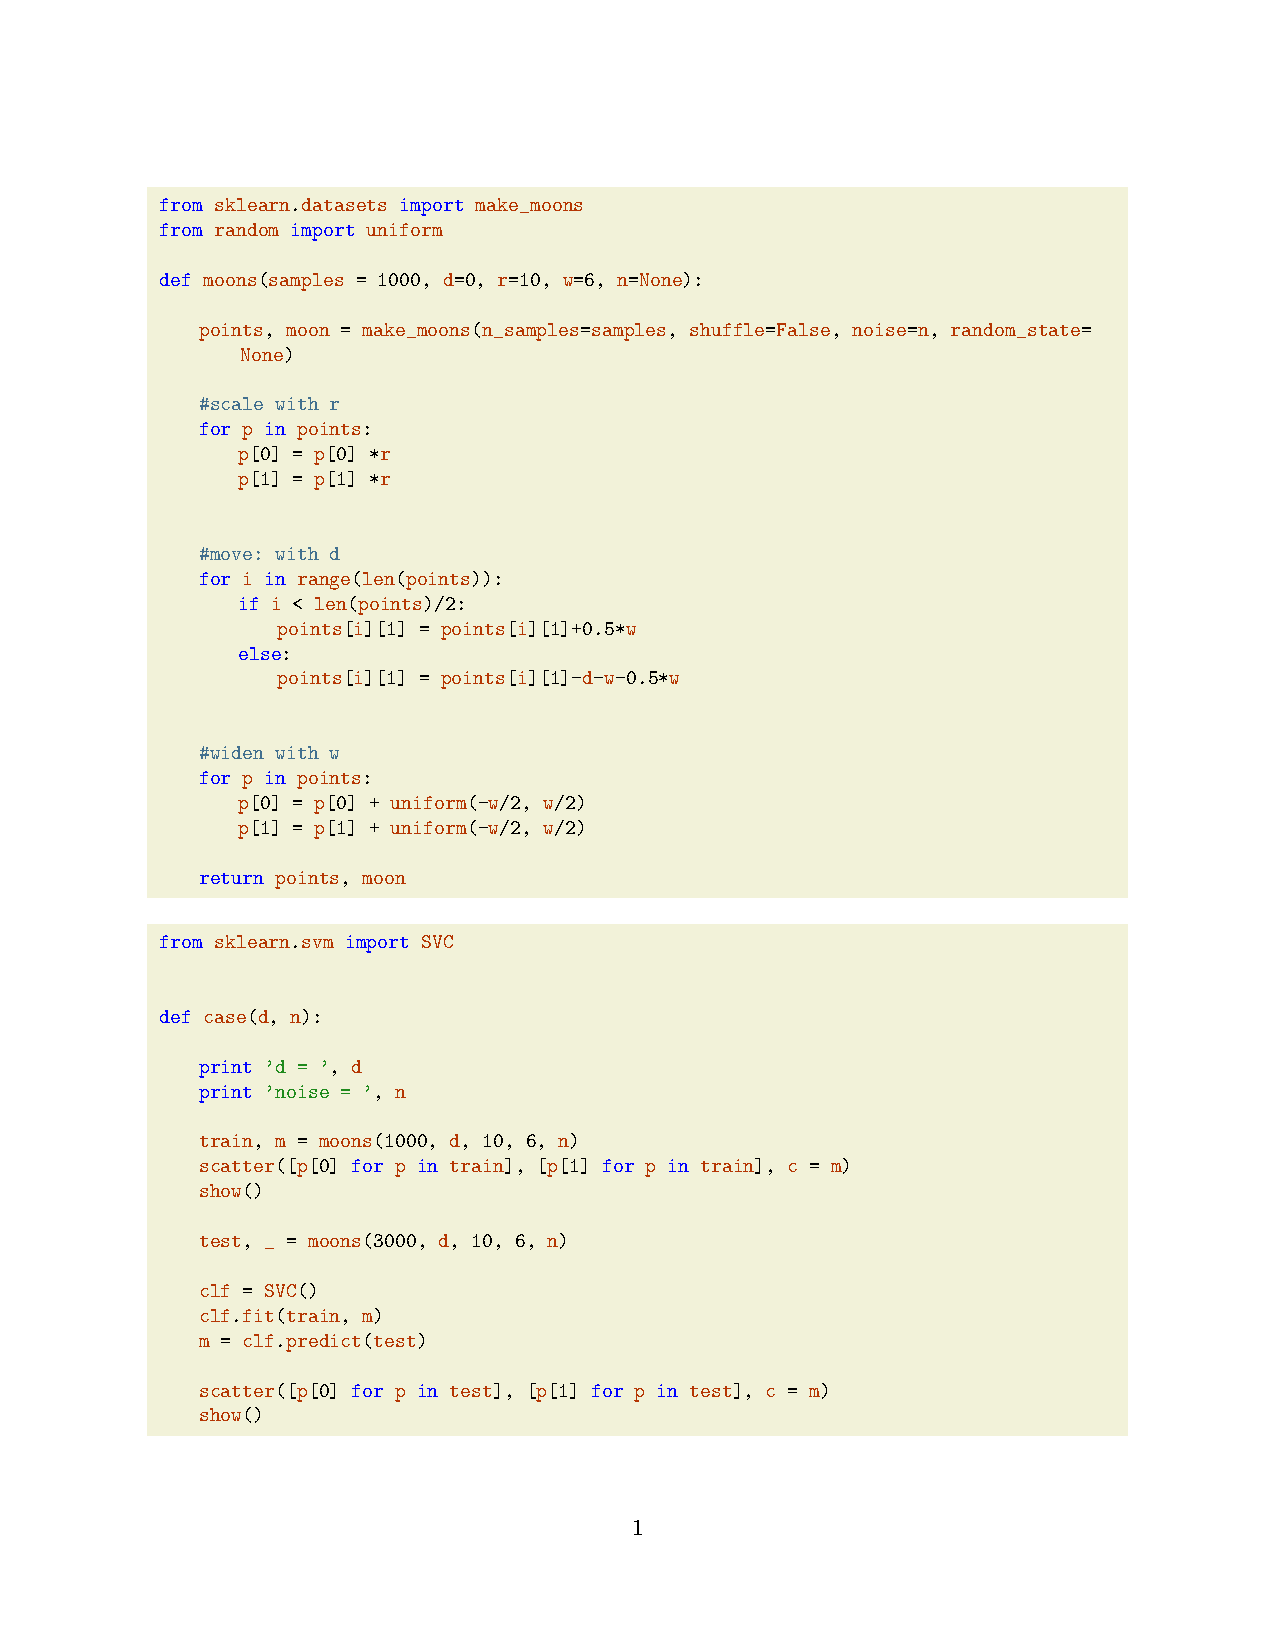
\includepdf[pages={1-},scale=1]{ex7.pdf}

%CONTENTS
%NOTES


%COPY AND PASTE FROM HERE

%\begin{enumerate}
% \item 
%\end{enumerate}

%\hyperref{link}{text}

%\begin[Language=Python]{lstlisting}
%#PYTHON CODE HERE
%\end{lstlisting}

%\lstinputlisting[Language=Python]{ }

%\begin{figure}
% \center
% \includegraphics[width= cm]{ }
% \caption{}
%\end{figure}

%BIBLIOGRPAHY?
\bibliographystyle{plain}%amsalpha
\bibliography{Top30.bib}
%\bibentry{}

\end{document}
